\normaltrue \difficilefalse \tdifficilefalse
\correctionfalse

%\UPSTIidClasse{11} % 11 sup, 12 spé
%\newcommand{\UPSTIidClasse}{12}

\exer{Pompe oscillante $\star$ \label{C2:06:13}}
\setcounter{numques}{0}
\UPSTIcompetence{C2-06}
\index{Compétence C2-06}
\index{Pompe oscillante}

\ifcorrection
\else
\textbf{Pas de corrigé pour cet exercice.}
\fi

\ifprof
\else
Soit le mécanisme suivant. On a $\vect{AB}=R\vect{i_1}$ et $\vect{CA}=H\vect{j_0}$. De plus, 
$R=\SI{10}{mm}$ et $H=\SI{60}{mm}$. Par ailleurs, on note $\vect{CB}=\lambda(t) \vect{i_2}$

\begin{center}
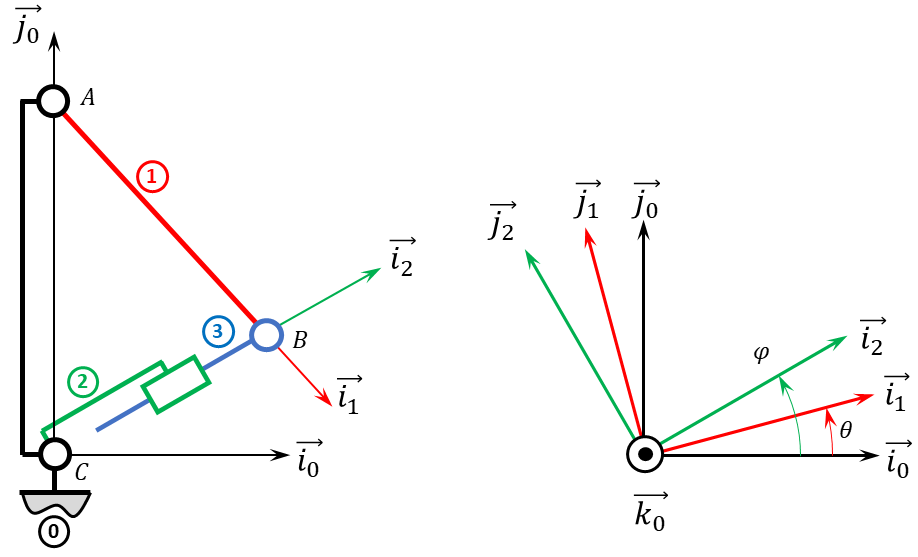
\includegraphics[width=\linewidth]{13_01}
\end{center}
\fi


\question{Tracer le graphe des liaisons.}
\ifprof
\else
\fi

\question{Exprimer $\lambda(t)$ en fonction de $\theta(t)$.}
\ifprof
\else
\fi

\question{Exprimer $\dot{\lambda}(t)$ en fonction de $\dot{\theta}(t)$.}
\ifprof
\else
\fi

\question{Exprimer le débit instantané de la pompe.}
\ifprof
\else
\fi

\question{En utilisant Python, donner le débit instantané de la pompe pour un tour de pompe pour un piston de diamètre $D=\SI{10}{mm}$.}
\ifprof
\else
\fi




\ifprof
\else
\begin{flushright}
\footnotesize{Corrigé  voir \ref{C2:06:13}.}
\end{flushright}%
\fi